\documentclass[a4paper,10pt,titlepage]{report}
\usepackage[utf8]{inputenc}
\usepackage[T1]{fontenc}
\usepackage[english]{babel}
\usepackage{amssymb}
\usepackage{amsmath}
\usepackage{amsthm}
\usepackage{graphicx}
\usepackage{fancyhdr}
\usepackage{lastpage}
\usepackage{pgfplots}
\usepackage{listings}
\usepackage{algorithm}
\usepackage{algpseudocode}
\usepackage{wrapfig}
\usepackage[document]{ragged2e}
\usepackage[margin=1in]{geometry}
\usepackage{enumitem}
\usepackage{color}
\usepackage{datenumber}
\usepackage{venndiagram}
\usepackage{chngcntr}
\setdatetoday
\addtocounter{datenumber}{0} 
\setdatebynumber{\thedatenumber}
\date{}
\setcounter{secnumdepth}{0}
\pagestyle{fancy}
\fancyhf{}


%lstlisting ting:
\definecolor{dkgreen}{rgb}{0,0.45,0}
\definecolor{gray}{rgb}{0.5,0.5,0.5}
\definecolor{mauve}{rgb}{0.30,0,0.30}
\lstset{frame=tb,
  language=C++,
  aboveskip=3mm,
  belowskip=3mm,
  showstringspaces=false,
  columns=flexible,
  basicstyle={\small\ttfamily},
  numbers=left,
  numberstyle=\footnotesize,
  keywordstyle=\color{dkgreen}\bfseries,
  commentstyle=\color{dkgreen},
  stringstyle=\color{mauve},
  frame=single,
  breaklines=true,
  breakatwhitespace=false
  tabsize=1
}
\renewcommand{\lstlistingname}{Code}

\newcommand{\Z}{\mathbb{Z}}
\lhead{Algorithms in Cheminformatics (DM840)}
\rhead{ Ilona Benko}
\rfoot{Page  \thepage \, of \pageref{LastPage}}
\counterwithin*{equation}{section}


\title{DM840 - mand 1}
\begin{document}
\begin{titlepage}
\centering
    \vspace*{9\baselineskip}
    \huge
    \bfseries
    2. Mandatory Assignment \\
    \normalfont
    Ilona Benko \\
  Ilben18 \\
	\huge
    Algorithms in Cheminformatics (DM840)  \\
    Daniel Merkle \\[4\baselineskip]
    \normalfont
	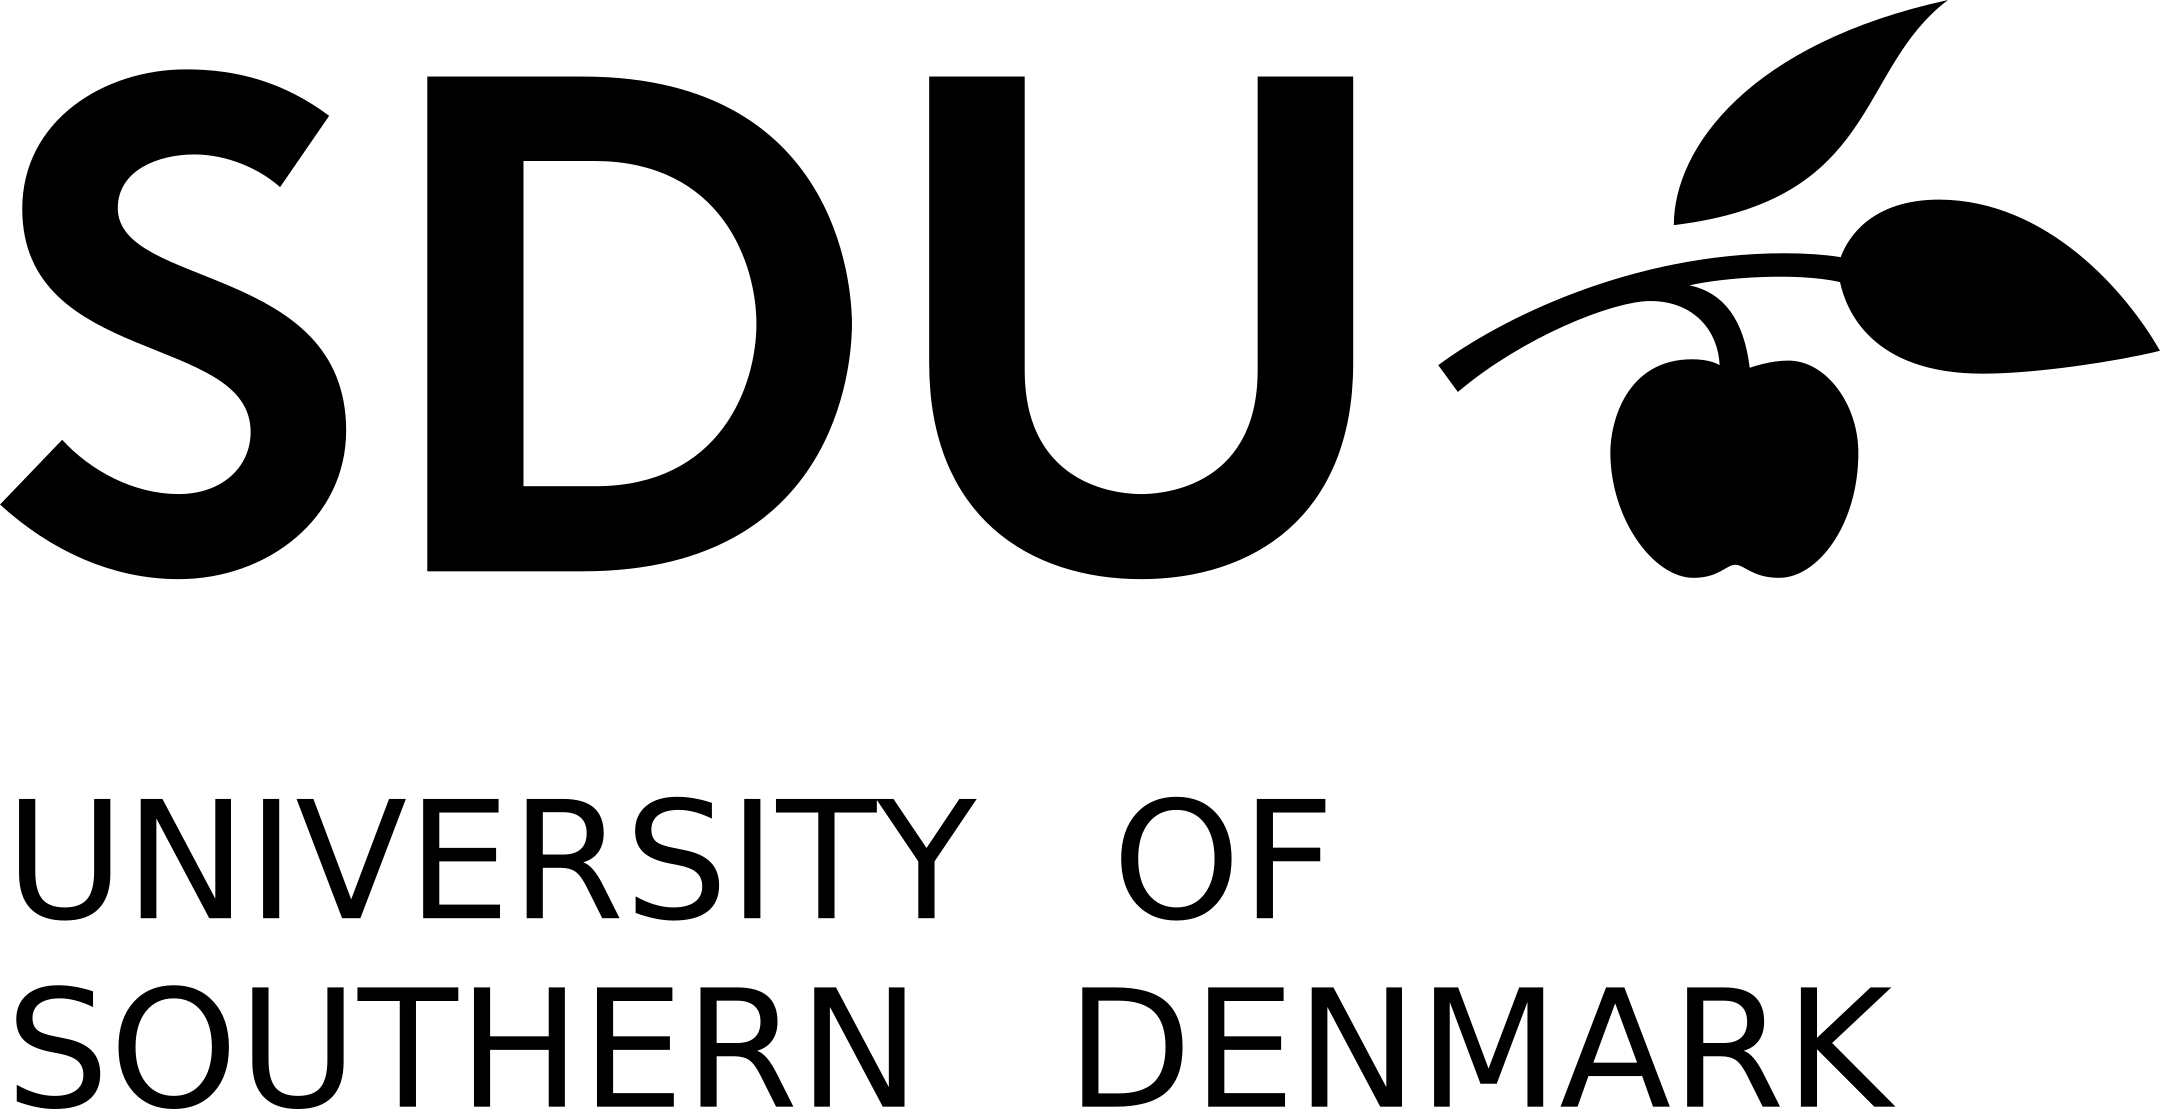
\includegraphics[scale=1]{SDU_logo}
    \vfill\
    \vspace{5mm}
    IMADA \\

    \textbf{\datedate}  \bf \\[2\baselineskip]
\end{titlepage}

\renewcommand{\thepage}{\roman{page}}% Roman numerals for page counter
\tableofcontents
\newpage
\setcounter{page}{1}
\renewcommand{\thepage}{\arabic{page}}
%https://www.overleaf.com/7644729885grfjqbyxxnbg

\section {Introduction}

In the second assignment for the course cheminformatics we were given a free choice of assignments, either two predefined projects or our own idea. We both originally planned on doing a custom project and got started on it but due to the close overlap with the microservices exam the plans had to be changed. \\

We ended up looking at the 2nd project for the assignment and begun on that. We decided for a first option which is Atom-Atom mapping. The main idea of this project is finding out how the size of a context in double pushout approach depends on two different parameters. Main goal was to construct an algorithm which does an enumeration of all graph grammar rules based on chemically valid mappings for a defined set of educts and products. Second step was to design a backtracking algorithm which includes previously mentioned and further more precisely  explained parameters. Unfortunately, due the lack of time, we brute forced only the first step and ended up with valid mappings but without doing it in a smart way. 

\section {Theory}

Previously in this course, we were introduced to the double pushout approach in modelling chemical reactions using graph grammar rules. This assignment is supposed to take this approach to a higher level by introducing chemically valid mappings.

\subsection{Chemically valid mapping}

Whenever there is some chemical reaction, we are introduced to a set of educts which transform to the set of products. During every chemical, some of the bonds between atoms in a set of educts are being destroyed and some new bonds are being formed with such molecules then creating a set of products. From the graph level of abstraction, we are just changing the way nodes are connected by deleting and adding some edges. This operations can be defined through 'mapping' by declaring where's the picture of every atom from educts graph in the products area.
\\
It's pretty much straightforward to see that educts are actually left hand-side in double pushout approach and products are the right side. Therefore, mappings of atoms directly lead to graph grammar rules. To be more exact, graph grammar rules can be formed only over chemically valid mappings. 

That means that the mapping needs to fulfill some constraints which are most easily trackable in the transition graph. Over there, we put all the atoms and bonds from both educts and products and we mark the bonds which are being broken with "X" and created bonds with "O".
\\
First important thing to notice is that such set of atoms and bonds forms a cycle. Secondly, marks of types of bonds in such cycle needs to be alternating, which means we are left only with cycles which have even number of nodes. When we think about what's happening between atoms on the energy level, this is logical because all systems tend to preserve as large as possible amount of energy. Also, charges are being passed between atoms with alternating change of sign so for a whole molecule to be balanced and reaction physically possible, even number of atoms must be included.
\\
Such mapping can then be called chemically valid and the even number of atoms from the cycle where changes appeared are put in the context of double pushout approach rule.
\\
Mathematically speaking, while performing such mapping, we are searching for subgraph isomorphisms. To define it, we firstly need to define what a morphism and monomorphism are.
\\
Graph morphism m between graphs G=(V, E), H=(V, E) with some vertices u, v $\in$ V can be defined as follows:
\begin{equation}
    \forall e = (u,v) \in E_g : m(e) = (m(u),m(v)) \in E_h
\end{equation}
Graph monomorphism is injective morphism:
\begin{equation}
    \forall u,v \in V_g, u \neq v \rightarrow m(u) \neq m(v)
\end{equation}
Subgraph isomorphism is monomorphism for which it holds:
\begin{equation}
    (u,v) \in E_g \Leftrightarrow (m(u),m(v)) \in E_h
\end{equation}
And finally, isomorphism is a subgraph isomorphism which is bijection of vertices, so each vertex with image in H has its original in G and there is unique mapping for every vertex from G to H.
\\
Whenever there are some graph transformation rules such as  double pushout rules p,$ p=(L\leftarrow K \tigharrow R)$, we have a situation that $L\setminus K$ is deleted, K is being preserved and $R\setminus K$ added and between L and K and R and K there is a monomorphism relation. Subgraph isomorphisms and isomorphisms are just more constrained cases of the same relations. 
\\
While performing atom to atom mappings, there can be several from which all are chemically valid. When such pair of different mapping leads to identical graph grammar rule, we are talking about isomorphisms or automorphisms and when it leads to different rules we have subgraph isomorphisms. 

\subsection{Partial chemically valid mapping}

General case of chemically valid mapping is described above. The problem is that it may be too general for some appliances, so parameters k and c are introduced.
In the case of chemically valid mapping in previous subsection, when only atoms from the cycle are put into the context, k=0. Parameter k represents the distance between different nodes which are added to the context in regard to those nodes which are part of the cycle forming the context when k=0. When k=1, all nodes which are one edge away from the cycle are also put in the context, when k=2, nodes which are two edges away are added to the context and so on. Edges connecting them are also being added, no matter if they were part of educt or product graph. Because of some extra elements but basic cycle basis are being added to the context, this mapping is called partially chemically valid.
\\
Therefore, we can define k as an unlimited integer value, through in practice it's not likely it will grow for more than a factor ten and that only in a case of really big molecules. In cases we had to consider in this project, maximum value which k takes is two and the molecules we were working with weren't completely trivial regarding number of atoms. 
\\
Introducing k is one way of creating some extra restrictions to the rule, as those nodes with exact bonds between the then need to also be found in both left-hand and right-hand sides i.e. educts and products. By that we are reducing the number of reactions the same rule can be applied to. 
\\
Another introduced parameter which can define some extra restrictions is c which represents the number of atoms forming the cycle basis of context. By definition of chemically valid mappings, c an only be even and minimum size to have a cycle in undirected graph without an edge weights is 4. Also, it is pretty unlikely to have a cycle with more than six atoms in organic molecules because of the binding (reactive) properties of carbon. 

\section {Implementation}

Starting point in implementing this is to find chemically valid mappings by adding into context only atoms which are forming the main cycle basis where changes are happening. From such algorithm, rules could be extracted and then set of different rules would form a generalization for finding isomorphisms. In our implementation this was brute forced. Second step would be including parameters k and c which would then form a complete set of rules and also require much more of computational time. 


\subsection{Environment}
Out environment for testing and running the code resulted in a small pipeline, The pipeline consisted of the tools git and jenkins. When we pushed our code to git it ssh'ed into logon.sdu.dk and further into a terminal room machine where it ran the wrapper file, we modified the wrapper file to use the python front end as we found it easier to use that as our interface for calling the function with all the arguments.
\\
we just the default way of building the code using the makefile, it was however considered highly if a CMakeFile should be created to allow for direct interaction with the MØD library, however MØD proved to be more time consuming then expected to install which meant this idea was scrapped and the git/jenkins/terminal room solution was used.
\\


\subsection {Code solution}

Our python front end included lists of all our educts and products for each of our reactions, these were simply passed to our function and the output was printed to the latex file.
\begin{lstlisting}
g1 = [smiles("OCC=O")]
g2 = [smiles("OC=CO")]
...
g5 = [smiles("O"), smiles("Cl"), smiles("CC(=O)OCC")]
g6 = [smiles("Cl"), smiles("OCC"), smiles("CC(=O)O")]
...
g13 = [smiles("OP(=O)(O)OP(=O)(O)O"), smiles("O")]
g14 = [smiles("O=P(O)(O)O"), smiles("O=P(O)(O)O")]

g15 = [smiles("C#N"), smiles("C#N")]
g16 = [smiles("N=CC#N")]

res1 = doStuff(g1, g2, 1 )
...
res8 = doStuff(g15, g16, 8)

allres = [res1, res2, res3, res4, res5, res6, res7, res8]

p = GraphPrinter()
p.withIndex = True

for a in inputGraphs: a.print()

for res in allres:
    for a in res:
        a.print(p)
        print(a.getGMLString())
\end{lstlisting}


Our Cpp code is quite simple, there is an empty space were our generic solution would have been if we had more time, but instead there's 8 "reactions" hard coded into our result. we got the solution just not in the right manner. we did use the original function to map an educt node to a product node.
\begin{lstlisting}
    // WORK AREA: START
    //
    std::vector <VertexMap> vertexMaps;
    // this is example code and probably only works when the example graphs are loaded
    VertexMap vertexMap;
    auto setById = [&vertexMap, &gEduct, &gProduct](std::size_t idEduct, std::size_t idProduct) {
      vertexMap.insert(VertexMap::value_type(getVertexFromId(idEduct, gEduct), getVertexFromId(idProduct, gProduct)));
    };

    if (reaction == 0) {
        //TODO Idea 1 (Probably a smarter way of doing it)
        //TODO 1. Find the larges sub graph isomorphism
        //TODO 2. Map the nodes within this.
        //TODO 3. recurse with smaller and smaller set until all nodes are mapped.

        //TODO Idea 2 (Brute force)
        //TODO Iterate over all possible mappings
        //TODO generate a list of rules.
        //TODO Eliminate all but the rule that changes the fewest bonds

    } else if (reaction == 8) {

....

    } else if (reaction == 5) {
        setById(0, 0);
        setById(1, 1);
        setById(2, 2);
        setById(3, 3);
        setById(4, 4);
        setById(5, 5);
        setById(6, 6);
        setById(7, 7);
        setById(8, 22);
        setById(9, 8);
        setById(10, 9);
        setById(11, 10);
        setById(12, 11);
        setById(13, 12);
        setById(14, 13);
        setById(28, 23);
        setById(15, 27);
        setById(16, 14);
        setById(17, 15);
        setById(18, 17);
        setById(19, 18);
        setById(20, 19);
        setById(21, 20);
        setById(22, 16);
        setById(23, 21);
        setById(24, 24);
        setById(25, 25);
        setById(26, 26);
        setById(27, 28);

        vertexMaps.push_back(vertexMap);

    } else if (reaction == 4) {
...
    // WORK AREA: END

\end{lstlisting}


\section {Results}

We solved everything, maybe not the correct way of doing it but we solved them all. The run timer to solve them was O(1) \newline
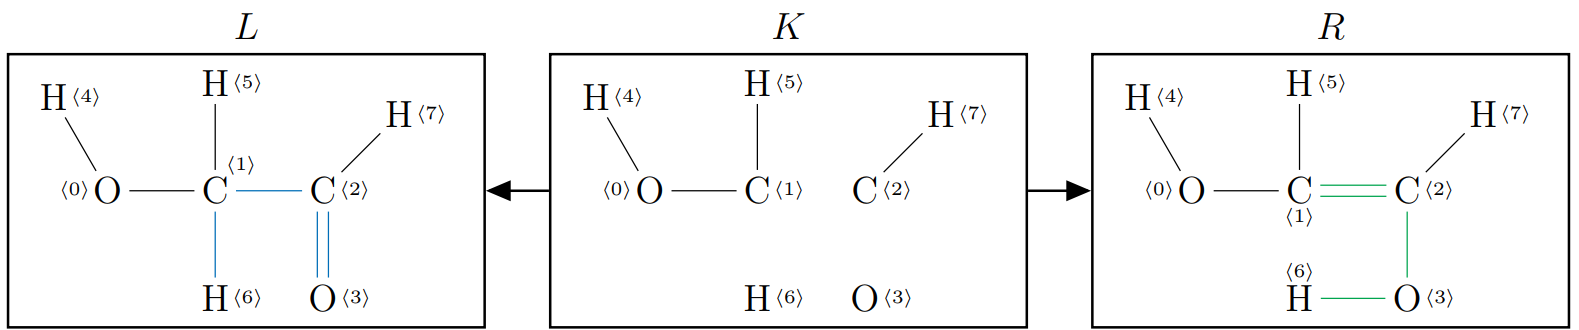
\includegraphics[scale=0.2]{a2_1.png}

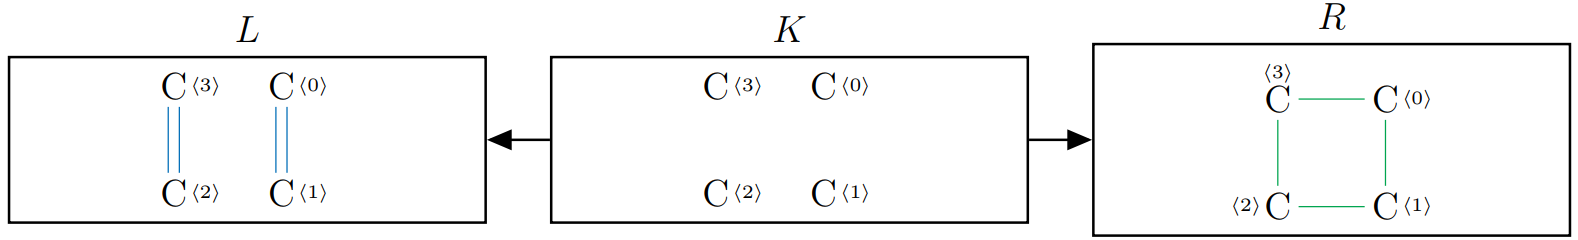
\includegraphics[scale=0.2]{a2_2.png}

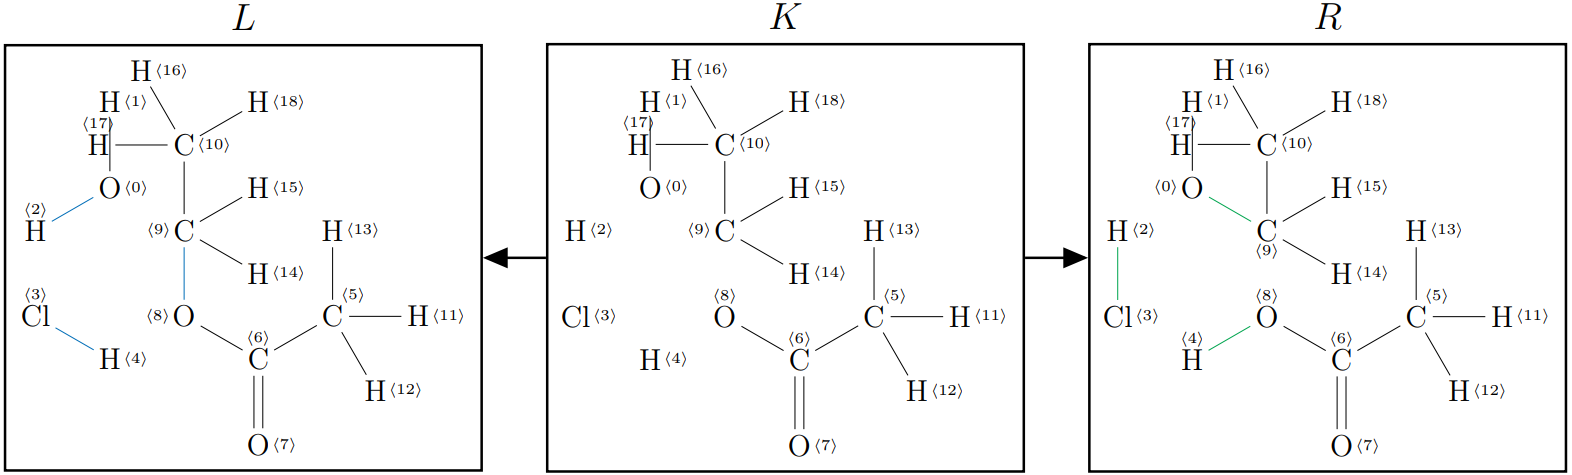
\includegraphics[scale=0.2]{a2_3.png}

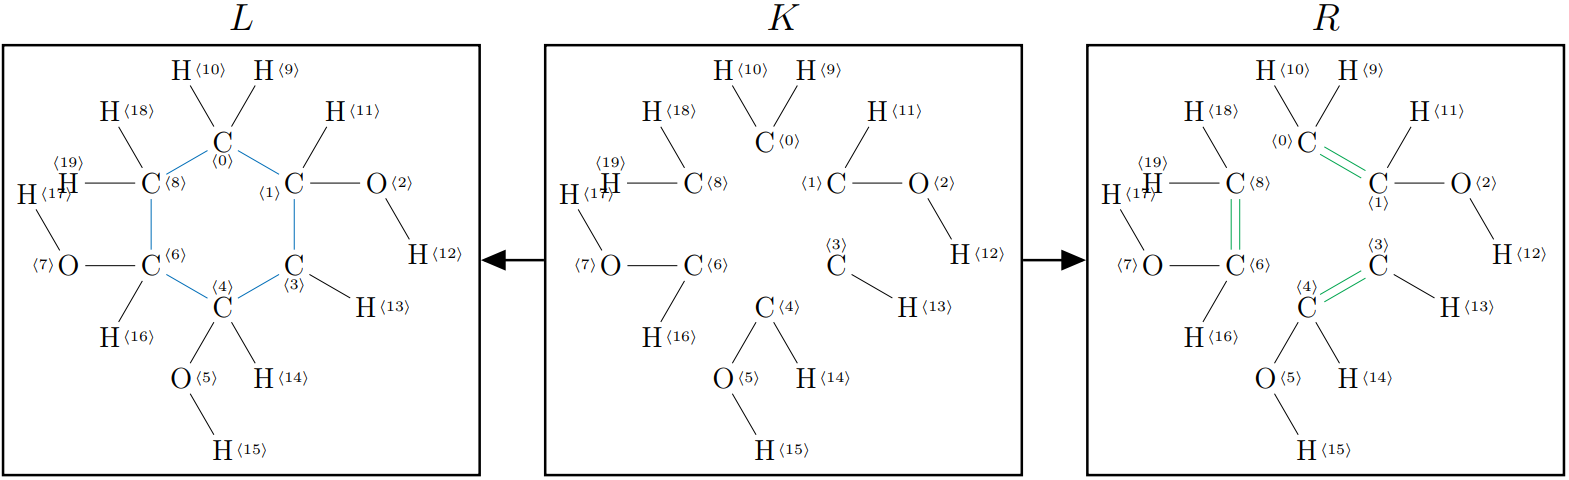
\includegraphics[scale=0.2]{a2_4.png}

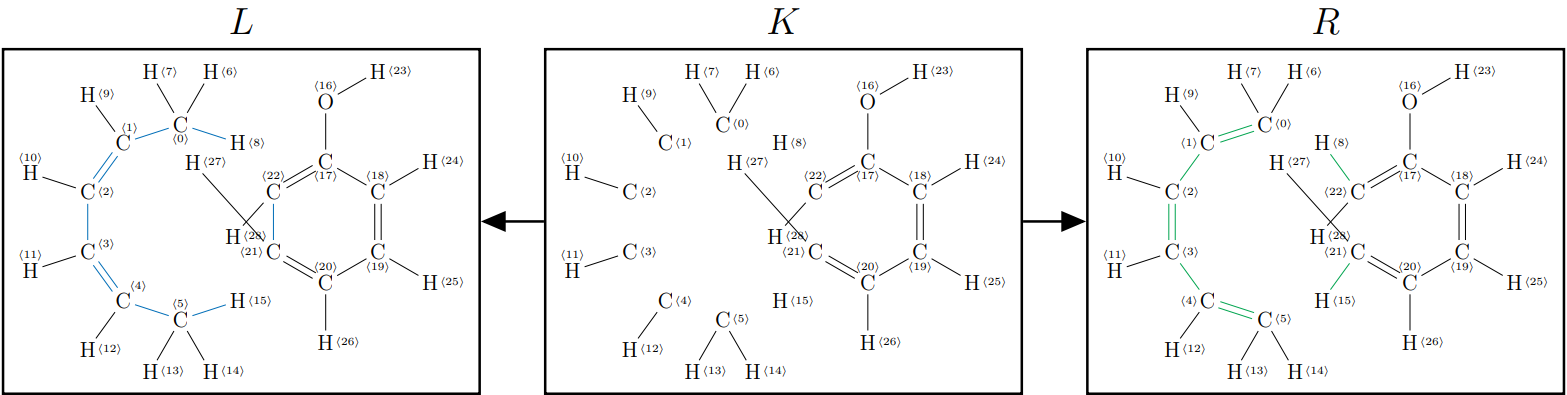
\includegraphics[scale=0.2]{a2_5.png}

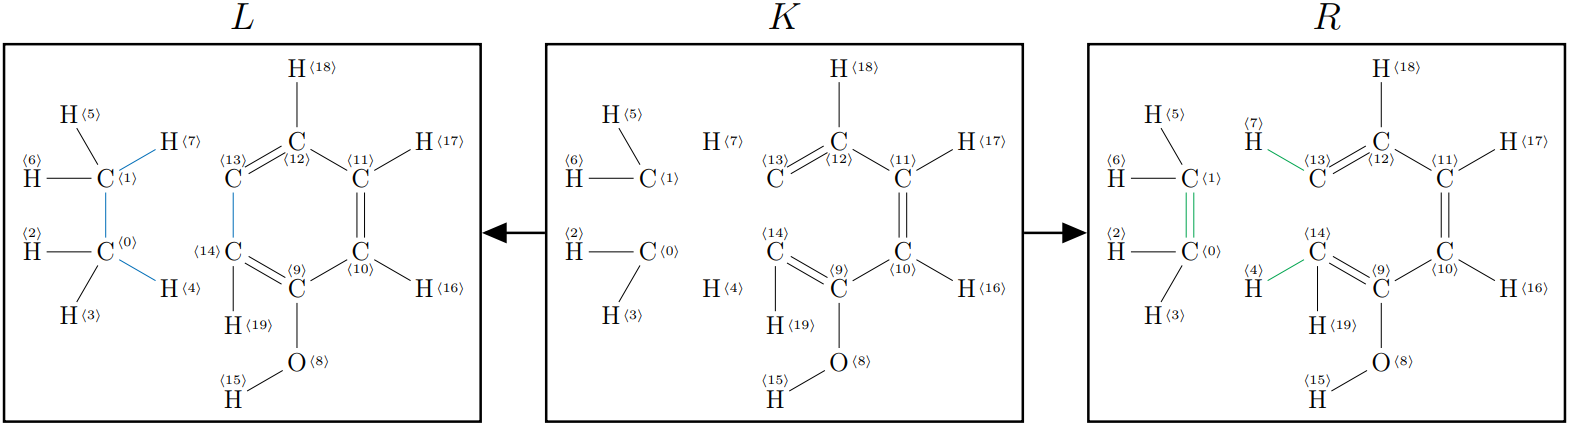
\includegraphics[scale=0.2]{a2_6.png}

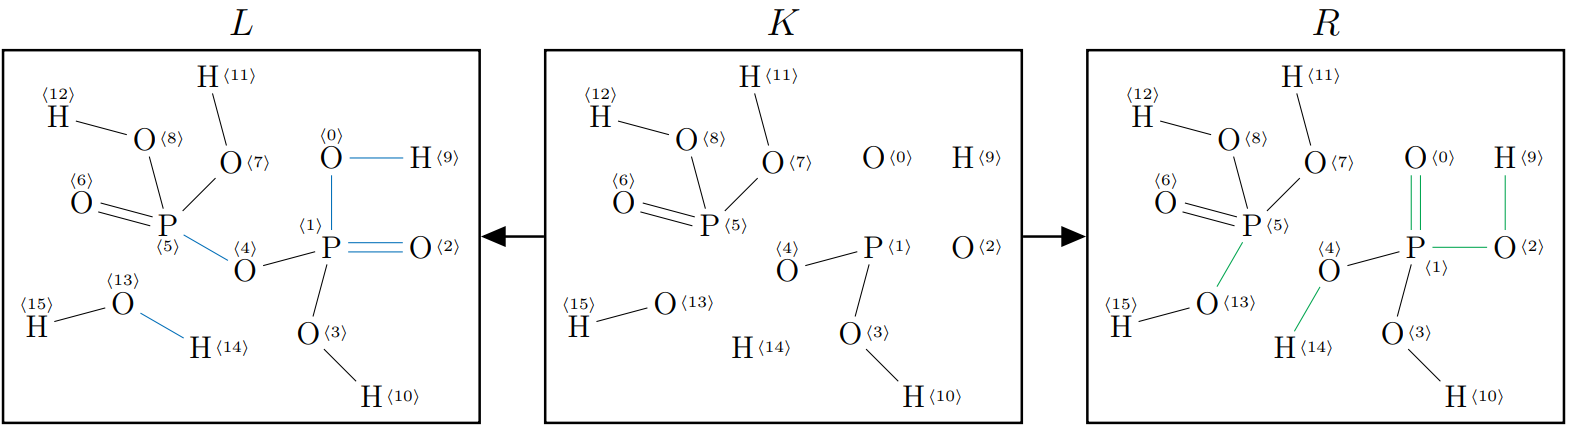
\includegraphics[scale=0.2]{a2_7.png}

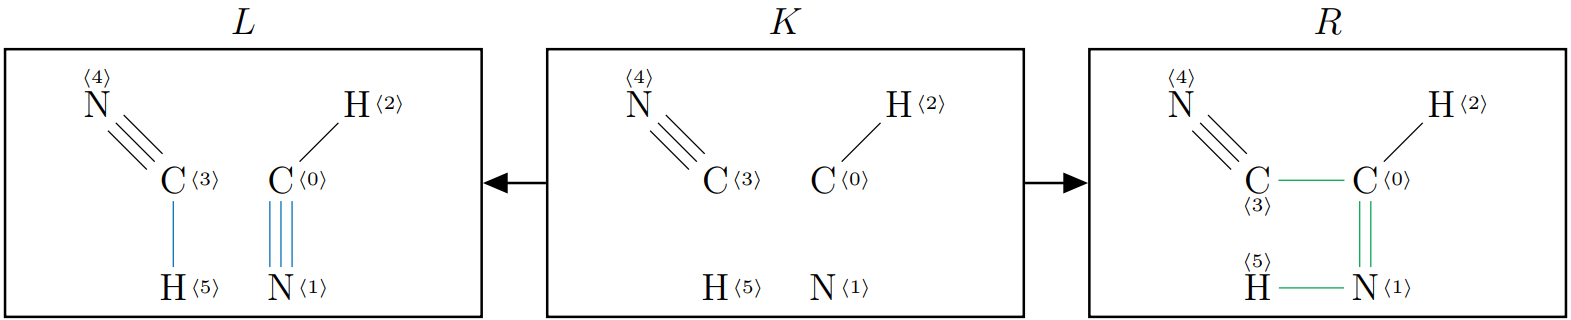
\includegraphics[scale=0.2]{a2_8.png}


\begin{table}[!htb]
  \centering
  \begin{tabular}{ll|cccc}\\
    Educts & Products & $k$ & $c$ & $n$ & $t$\\\hline
    C=C, C=C & C1CCC1 & 0 & 4 & & \\
    C=C, C=C & C1CCC1 & 1 & 4 & & \\
    O, Cl, CC(=O)OCC & Cl, OCC, CC(=O)O & 0 & 6 \\
    O, Cl, CC(=O)OCC & Cl, OCC, CC(=O)O & 1 & 6 \\
    O, Cl, CC(=O)OCC & Cl, OCC, CC(=O)O & 2 & 6 \\
    C1C(O)CC(O)C(O)C1 & C=CO, C=CO, C=CO  & 0 & 6 & & \\
    C1C(O)CC(O)C(O)C1 & C=CO, C=CO, C=CO  & 1 & 6 & & \\
    CC=CC=CC, OC1C=CC=CC=1 & C=CC=CC=C, OC(=C)C=CC=C & 0 & 6 & & \\
    CC=CC=CC, OC1C=CC=CC=1 & C=CC=CC=C, OC(=C)C=CC=C & 1 & 6 & & \\
    CC=CC=CC, OC1C=CC=CC=1 & C=CC=CC=C, OC(=C)C=CC=C & 2 & 6 & & \\
    CC, OC1C=CC=CC=1 & C=C, OC(=C)C=CC=C & 0 & 6 & & \\
    CC, OC1C=CC=CC=1 & C=C, OC(=C)C=CC=C & 1 & 6 & & \\
    CC, OC1C=CC=CC=1 & C=C, OC(=C)C=CC=C & 2 & 6 & & \\
    OP(=O)(O)OP(=O)(O)O, O & O=P(O)(O)O, O=P(O)(O)O  & 0 & 4 & & \\
    OP(=O)(O)OP(=O)(O)O, O & O=P(O)(O)O, O=P(O)(O)O  & 1 & 4 & & \\
    OP(=O)(O)OP(=O)(O)O, O & O=P(O)(O)O, O=P(O)(O)O  & 0 & 6 & & \\
    OP(=O)(O)OP(=O)(O)O, O & O=P(O)(O)O, O=P(O)(O)O  & 1 & 6 & & \\
    C\#N, C\#N & N=CC\#N & 0 & 4 & & \\
    C\#N, C\#N & N=CC\#N & 1 & 4 & & \\
 \end{tabular}
\end{table}
\newpage
In this table the parameters k and c are defined as described above, n is the number of different graph grammar rules you found, and t is the number of different mappings that were supposed to be created in order to find some number (t) of equivalent different graph grammar rules, i.e. On the implementation level, t is represented as the number of calls to vertexMaps.pushback(vertexMap). 

\section {Limitations}
The current limitation of the code is that it does not support k and c, and simply returns a hard coded solution to the problem, a few different ways of solving the problem the correct way is however discussed in the discussion section. 

\section{Discussion}
Due to rather poor planning we ended up not having time to implement the solutions, We ending up discussing two possible solutions to the project.

\subsection{Idea 1 (Brute force)}
The brute force way of solving the problem would simply just generate all possible mappings for all the labels. eg. all carbons maps to all carbons. when all rules have been generated we'll want to look for the "ruleset" with the fewest changes to bonds. and return this as our result. this would create a runtime of NP Complete. Note that finding a graph morphisms, monomorphisms, subgraph isomorphisms and isomorphisms are all NP Complete problems so this was expected.  
The Algortihm would look like the following
This function to generate all mappings would look something like this.
\begin{lstlisting}
def mapping_function([]educt_nodes,[]product_nodes)
        for node in educt_nodes
            for n in product_nodes
                if node.lable = n.lable
                    mapnode(node, n) //This should push to a global data type, or be handled via return.
                    if (educt_nodes.size = 1){
                    return:
                    }else{
                    mapping_function([]educt_nodes.remove(node),[]product_nodes.remove(n))
                    }
\end{lstlisting}
The function to select the mapping, It's pretty simply it just iterate over the rule, I assume MØD has a function for this. as it's the data type and if it doesn't some designer needs to add more basic functionality.
\begin{lstlisting}
def Select_best_rule([]Rule_list){
    rule smallest_rule.left.size = 2^64
    for rule in rule_list{
        if (rule.left.size < smallest_rule.left.size)
            smallest_rule = rule
    }    
    return smallest_rule
}
\end{lstlisting}
The main call of the algorithm would look something like this
\begin{lstlisting}
    global []Rules_list = []
    mapping_function(educt_nodes,product_nodes)
    return Select_best_rule(Rules_list)
\end{lstlisting}
        
\subsection{Idea 1 (Probably a smarter way of doing it)}
The second and better way of doing this would be to first find the larges sub graph isomorphism match. map all the nodes within this and recurse, This would most likely create a very good runtime. buy you could risk the program returning the wrong value due to wrong mappings happening. a work around for this would be to drop a sub graph isomorphism match size 2 and using the brute force method for the remaining missing matches and then eliminating all but the correct result.

for the algorithm we'd choose to implement something like listed in the paper Maximum Common Sub graph \footnote{Edmund Duesbury, John D. Holliday, Peter Willett, Maximum Common Subgraph: Http://match.pmf.kg.ac.rs/electronic_versions/Match77/n2/match77n2_213-232.pdf
}
We'd make the assumption that we can return the smallest sub graph with both ID's of the educt and product.
\begin{lstlisting}
def mapping(educt_sub_graph, product_sub_graph){
    remove_from_graph(educt_graph, educt_sub_graph)
    remove_from_graph(product_graph, product_sub_graph)
    for n in educt_sub_graph.size{
        map_to(product_graph.canonicalorder.id(n), educt_graph.canonicalorder.id(n))
    return
    }
}
\end{lstlisting}

\section{Appexdix}

The returned solutions by the program, the id's for the first reaction is 0 and 2, and for the rest it's the id+1

\begin{lstlisting}
rule [
	ruleID "r_{0}"
	left [
		edge [ source 2 target 1 label "-" ]
		edge [ source 3 target 2 label "=" ]
		edge [ source 6 target 1 label "-" ]
	]
	context [
		node [ id 0 label "O" ]
		node [ id 1 label "C" ]
		node [ id 2 label "C" ]
		node [ id 3 label "O" ]
		node [ id 4 label "H" ]
		node [ id 5 label "H" ]
		node [ id 6 label "H" ]
		node [ id 7 label "H" ]
		edge [ source 1 target 0 label "-" ]
		edge [ source 4 target 0 label "-" ]
		edge [ source 5 target 1 label "-" ]
		edge [ source 7 target 2 label "-" ]
	]
	right [
		edge [ source 2 target 1 label "=" ]
		edge [ source 3 target 2 label "-" ]
		edge [ source 6 target 3 label "-" ]
	]
]
rule [
	ruleID "r_{1}"
	left [
		edge [ source 1 target 0 label "-" ]
		edge [ source 2 target 1 label "=" ]
		edge [ source 3 target 0 label "-" ]
	]
	context [
		node [ id 0 label "C" ]
		node [ id 1 label "C" ]
		node [ id 2 label "O" ]
		node [ id 3 label "H" ]
	]
	right [
		edge [ source 1 target 0 label "=" ]
		edge [ source 2 target 1 label "-" ]
		edge [ source 3 target 2 label "-" ]
	]
]
rule [
	ruleID "r_{3}"
	left [
		edge [ source 1 target 0 label "=" ]
		edge [ source 3 target 2 label "=" ]
	]
	context [
		node [ id 0 label "C" ]
		node [ id 1 label "C" ]
		node [ id 2 label "C" ]
		node [ id 3 label "C" ]
	]
	right [
		edge [ source 1 target 0 label "-" ]
		edge [ source 3 target 2 label "-" ]
		edge [ source 2 target 1 label "-" ]
		edge [ source 3 target 0 label "-" ]
	]
]
WARNING: No viable geometries for Cl with bonds S = 1.
rule [
	ruleID "r_{4}"
	left [
		edge [ source 2 target 0 label "-" ]
		edge [ source 4 target 3 label "-" ]
		edge [ source 9 target 8 label "-" ]
	]
	context [
		node [ id 0 label "O" ]
		node [ id 1 label "H" ]
		node [ id 2 label "H" ]
		node [ id 3 label "Cl" ]
		node [ id 4 label "H" ]
		node [ id 5 label "C" ]
		node [ id 6 label "C" ]
		node [ id 7 label "O" ]
		node [ id 8 label "O" ]
		node [ id 9 label "C" ]
		node [ id 10 label "C" ]
		node [ id 11 label "H" ]
		node [ id 12 label "H" ]
		node [ id 13 label "H" ]
		node [ id 14 label "H" ]
		node [ id 15 label "H" ]
		node [ id 16 label "H" ]
		node [ id 17 label "H" ]
		node [ id 18 label "H" ]
		edge [ source 1 target 0 label "-" ]
		edge [ source 7 target 6 label "=" ]
		edge [ source 6 target 5 label "-" ]
		edge [ source 8 target 6 label "-" ]
		edge [ source 10 target 9 label "-" ]
		edge [ source 11 target 5 label "-" ]
		edge [ source 12 target 5 label "-" ]
		edge [ source 13 target 5 label "-" ]
		edge [ source 14 target 9 label "-" ]
		edge [ source 15 target 9 label "-" ]
		edge [ source 16 target 10 label "-" ]
		edge [ source 17 target 10 label "-" ]
		edge [ source 18 target 10 label "-" ]
	]
	right [
		edge [ source 2 target 3 label "-" ]
		edge [ source 9 target 0 label "-" ]
		edge [ source 4 target 8 label "-" ]
	]
]
WARNING: No viable geometries for Cl with bonds S = 1.
WARNING: No viable geometries for Cl with bonds S = 1.
rule [
	ruleID "r_{5}"
	left [
		edge [ source 1 target 0 label "-" ]
		edge [ source 3 target 1 label "-" ]
		edge [ source 4 target 3 label "-" ]
		edge [ source 6 target 4 label "-" ]
		edge [ source 8 target 0 label "-" ]
		edge [ source 8 target 6 label "-" ]
	]
	context [
		node [ id 0 label "C" ]
		node [ id 1 label "C" ]
		node [ id 2 label "O" ]
		node [ id 3 label "C" ]
		node [ id 4 label "C" ]
		node [ id 5 label "O" ]
		node [ id 6 label "C" ]
		node [ id 7 label "O" ]
		node [ id 8 label "C" ]
		node [ id 9 label "H" ]
		node [ id 10 label "H" ]
		node [ id 11 label "H" ]
		node [ id 12 label "H" ]
		node [ id 13 label "H" ]
		node [ id 14 label "H" ]
		node [ id 15 label "H" ]
		node [ id 16 label "H" ]
		node [ id 17 label "H" ]
		node [ id 18 label "H" ]
		node [ id 19 label "H" ]
		edge [ source 2 target 1 label "-" ]
		edge [ source 5 target 4 label "-" ]
		edge [ source 7 target 6 label "-" ]
		edge [ source 9 target 0 label "-" ]
		edge [ source 10 target 0 label "-" ]
		edge [ source 11 target 1 label "-" ]
		edge [ source 12 target 2 label "-" ]
		edge [ source 13 target 3 label "-" ]
		edge [ source 14 target 4 label "-" ]
		edge [ source 15 target 5 label "-" ]
		edge [ source 16 target 6 label "-" ]
		edge [ source 17 target 7 label "-" ]
		edge [ source 18 target 8 label "-" ]
		edge [ source 19 target 8 label "-" ]
	]
	right [
		edge [ source 1 target 0 label "=" ]
		edge [ source 4 target 3 label "=" ]
		edge [ source 8 target 6 label "=" ]
	]
]
rule [
	ruleID "r_{6}"
	left [
		edge [ source 1 target 0 label "-" ]
		edge [ source 2 target 1 label "=" ]
		edge [ source 3 target 2 label "-" ]
		edge [ source 4 target 3 label "=" ]
		edge [ source 5 target 4 label "-" ]
		edge [ source 8 target 0 label "-" ]
		edge [ source 15 target 5 label "-" ]
		edge [ source 22 target 21 label "-" ]
	]
	context [
		node [ id 0 label "C" ]
		node [ id 1 label "C" ]
		node [ id 2 label "C" ]
		node [ id 3 label "C" ]
		node [ id 4 label "C" ]
		node [ id 5 label "C" ]
		node [ id 6 label "H" ]
		node [ id 7 label "H" ]
		node [ id 8 label "H" ]
		node [ id 9 label "H" ]
		node [ id 10 label "H" ]
		node [ id 11 label "H" ]
		node [ id 12 label "H" ]
		node [ id 13 label "H" ]
		node [ id 14 label "H" ]
		node [ id 15 label "H" ]
		node [ id 16 label "O" ]
		node [ id 17 label "C" ]
		node [ id 18 label "C" ]
		node [ id 19 label "C" ]
		node [ id 20 label "C" ]
		node [ id 21 label "C" ]
		node [ id 22 label "C" ]
		node [ id 23 label "H" ]
		node [ id 24 label "H" ]
		node [ id 25 label "H" ]
		node [ id 26 label "H" ]
		node [ id 27 label "H" ]
		node [ id 28 label "H" ]
		edge [ source 6 target 0 label "-" ]
		edge [ source 7 target 0 label "-" ]
		edge [ source 9 target 1 label "-" ]
		edge [ source 10 target 2 label "-" ]
		edge [ source 11 target 3 label "-" ]
		edge [ source 12 target 4 label "-" ]
		edge [ source 13 target 5 label "-" ]
		edge [ source 14 target 5 label "-" ]
		edge [ source 17 target 16 label "-" ]
		edge [ source 18 target 17 label "-" ]
		edge [ source 19 target 18 label "=" ]
		edge [ source 20 target 19 label "-" ]
		edge [ source 21 target 20 label "=" ]
		edge [ source 22 target 17 label "=" ]
		edge [ source 23 target 16 label "-" ]
		edge [ source 24 target 18 label "-" ]
		edge [ source 25 target 19 label "-" ]
		edge [ source 26 target 20 label "-" ]
		edge [ source 27 target 21 label "-" ]
		edge [ source 28 target 22 label "-" ]
	]
	right [
		edge [ source 1 target 0 label "=" ]
		edge [ source 2 target 1 label "-" ]
		edge [ source 3 target 2 label "=" ]
		edge [ source 4 target 3 label "-" ]
		edge [ source 5 target 4 label "=" ]
		edge [ source 8 target 22 label "-" ]
		edge [ source 15 target 21 label "-" ]
	]
]
rule [
	ruleID "r_{7}"
	left [
		edge [ source 1 target 0 label "-" ]
		edge [ source 4 target 0 label "-" ]
		edge [ source 7 target 1 label "-" ]
		edge [ source 14 target 13 label "-" ]
	]
	context [
		node [ id 0 label "C" ]
		node [ id 1 label "C" ]
		node [ id 2 label "H" ]
		node [ id 3 label "H" ]
		node [ id 4 label "H" ]
		node [ id 5 label "H" ]
		node [ id 6 label "H" ]
		node [ id 7 label "H" ]
		node [ id 8 label "O" ]
		node [ id 9 label "C" ]
		node [ id 10 label "C" ]
		node [ id 11 label "C" ]
		node [ id 12 label "C" ]
		node [ id 13 label "C" ]
		node [ id 14 label "C" ]
		node [ id 15 label "H" ]
		node [ id 16 label "H" ]
		node [ id 17 label "H" ]
		node [ id 18 label "H" ]
		node [ id 19 label "H" ]
		edge [ source 2 target 0 label "-" ]
		edge [ source 3 target 0 label "-" ]
		edge [ source 5 target 1 label "-" ]
		edge [ source 6 target 1 label "-" ]
		edge [ source 9 target 8 label "-" ]
		edge [ source 10 target 9 label "-" ]
		edge [ source 11 target 10 label "=" ]
		edge [ source 12 target 11 label "-" ]
		edge [ source 13 target 12 label "=" ]
		edge [ source 14 target 9 label "=" ]
		edge [ source 15 target 8 label "-" ]
		edge [ source 16 target 10 label "-" ]
		edge [ source 17 target 11 label "-" ]
		edge [ source 18 target 12 label "-" ]
		edge [ source 19 target 14 label "-" ]
	]
	right [
		edge [ source 1 target 0 label "=" ]
		edge [ source 4 target 14 label "-" ]
		edge [ source 7 target 13 label "-" ]
	]
]
rule [
	ruleID "r_{8}"
	left [
		edge [ source 2 target 1 label "=" ]
		edge [ source 1 target 0 label "-" ]
		edge [ source 5 target 4 label "-" ]
		edge [ source 9 target 0 label "-" ]
		edge [ source 14 target 13 label "-" ]
	]
	context [
		node [ id 0 label "O" ]
		node [ id 1 label "P" ]
		node [ id 2 label "O" ]
		node [ id 3 label "O" ]
		node [ id 4 label "O" ]
		node [ id 5 label "P" ]
		node [ id 6 label "O" ]
		node [ id 7 label "O" ]
		node [ id 8 label "O" ]
		node [ id 9 label "H" ]
		node [ id 10 label "H" ]
		node [ id 11 label "H" ]
		node [ id 12 label "H" ]
		node [ id 13 label "O" ]
		node [ id 14 label "H" ]
		node [ id 15 label "H" ]
		edge [ source 3 target 1 label "-" ]
		edge [ source 4 target 1 label "-" ]
		edge [ source 6 target 5 label "=" ]
		edge [ source 7 target 5 label "-" ]
		edge [ source 8 target 5 label "-" ]
		edge [ source 10 target 3 label "-" ]
		edge [ source 11 target 7 label "-" ]
		edge [ source 12 target 8 label "-" ]
		edge [ source 15 target 13 label "-" ]
	]
	right [
		edge [ source 2 target 1 label "-" ]
		edge [ source 1 target 0 label "=" ]
		edge [ source 14 target 4 label "-" ]
		edge [ source 9 target 2 label "-" ]
		edge [ source 13 target 5 label "-" ]
	]
]
WARNING: No viable geometries for N with bonds T = 1.
WARNING: No viable geometries for N with bonds T = 1.
rule [
	ruleID "r_{9}"
	left [
		edge [ source 1 target 0 label "#" ]
		edge [ source 5 target 3 label "-" ]
	]
	context [
		node [ id 0 label "C" ]
		node [ id 1 label "N" ]
		node [ id 2 label "H" ]
		node [ id 3 label "C" ]
		node [ id 4 label "N" ]
		node [ id 5 label "H" ]
		edge [ source 2 target 0 label "-" ]
		edge [ source 4 target 3 label "#" ]
	]
	right [
		edge [ source 1 target 0 label "=" ]
		edge [ source 3 target 0 label "-" ]
		edge [ source 5 target 1 label "-" ]
	]
]
\end{lstlisting}

\end{document}
